\chapter{Concept}
\label{sec:concept}

 % SELECTION APPLICATION, QUADTREE, USERSTUDY, VERGLEICHS-MAß

The goal of this work was to describe and implement a framework that allows for meaningful statements about differences between user selected regions of importance and computer generated mesh saliency maps to be made. It also included such a comparison on a basic, conceptual level. Based on these abstract tasks given, the workload and how I approached it, can be described by the following milestone-like, high level requirements.

\begin{enumerate*}
	\item implement a selection application for the V2C's projection installation
	\begin{enumerate*}
		\item spatial indexing of 3D data
		\item selection process
	\end{enumerate*}
	\item conduct a user study to acquire data for a comparison
	\item conceptualise a measure of similarities and differences between the data sets
\end{enumerate*}

In this section, I will go through these requirements and describe in more detail what specific challenges they entailed and how I went about implementing solutions to them. I will also describe the underlaying concepts I chose to use and how I amended them to better fit this work where needed.

	\subsection{Implementing a selection application for the V2C's projection installation}
	\label{sec:implementing_selection_application_v2c}
	% LRT = leibinz supercomputing centre(?)
One of the biggest challenges of this work was developing a piece of C++ software that allows users in the five-sided projection installation of the Leibniz Supercomputing Centre to select vertices of 3D objects using the existing soft- and hardware components at hand there. Designing, implementing and adjusting this software to being executable as a multi-threaded client-server application on the projection installation this software, was a challenging and time-consuming aspect of this work. For the rest of this work, this piece of software will be refferend to as \textit{selection application}. For details on its implementation, see section \ref{sec:selection_application}.

		\subsection{Spatial indexing of 3D data}
		\label{sec:impl_spatial_indexing_3d}
3D objects and data in general is read by compouters as lists of coordinates. Common 3D file formats such as .OBJ, .FBX and .STL contain the same data in similar structures, using multiple lists of different kinds of geometric information. While they these formats vary in the range of information they can hold, they all represent at least the following types of essential data. \textit{Vertices}, or a three tuple of float values describing x, y and zu coordinates and \textit{faces}, or basic triangles consisting of three vertices. Other optinal information that can be represented include vertex normals, texture coordinates and more complex features such as assigned materials, animations and armature objects. Figure \ref{fig:obj_content} shows an excerpt of a 3D file in .OBJ format, viewed in a simple text editor (gedit).

\begin{figure}[htb]
  \centering
  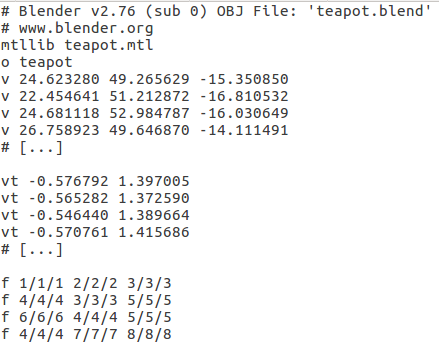
\includegraphics[width=.6\textwidth]{obj_content.png}\\ % PNG-File
  \caption{Notation in .OBJ format}\label{fig:obj_content}
\end{figure}

All these types of information share the following properties which were of relevance for this work. They are contiguous lists of lines, each line representing one instance of the data type indicated in the beginning of the line. Figure \ref{fig:obj_content} depicts an excerpt of an .OBJ file ocntaining vertices (lines starting with v), vertex textures (lines starting wit vt) and faces (lines starting with f).

These lists are not ordered. Depending on the modelling process, the vertices, faces and all the other attributes can be presented in an completely arbitrary order which hold very little information about the actual, geometric features of the object. The spatial position of any given vertex in relation to the entire object can not be retrieved from this type of notation. This created the demand for spatially indexing of 3D data in the scope this work.

I decided to implement the concept of Octrees \cite{Octree} because of its convenient characteristics as well as prior, personal working experience with \textit{quadtrees}. In an octree, the geometric size of the smallest possible leaf node can be determined in direct relation to the object to be indexed and, at any level, all leafs and nodes will be of the same size. This is highly useful in radius-based proximity-requests for multipl reasons as described in section \ref{sec:addVerticesToSelectionByCoordinates()}.

% @TODO hier gehts weiter	
% Reihenfolge, nicht wichtig und so!
